\chapter{Minimización de AFD}

\section{Minimización de un AFD. AFD equivalentes}

\textbf{Definición: }Dos AFD definidos sobre un alfabeto $I$, se dice equivalentes si ambos reconocen el mismo lenguaje.

Formalmente:

$D_1$ es equivalente a $D_2$ sobre $I$ si $L(D_1)=L(D_2)$

\section{Método de Comprobación}

Sean los autómatas $D_1=(S_1,I,\delta_1,s_1^*,F_1)$ y $D_2=(S_2,I,\delta_2,s_2^*,F_2)$

\begin{enumerate}
\item Unirlos en un único autómata determinista de modo que no sea conexo, como sigue:

$D=D_1\cup D_2=(S_1\cup S_2,I,\delta,s^*,F_1\cup F_2)$

donde :

$\delta(s,a)=\left\{ \begin{array}{ll} 
\delta_1(s,a) 	&	s\in S_1	\\
\delta_2(s,a)	& 	s\in S_2	\end{array}\right.$

Para $s^*$, podemos elegir $s_1^*$ o $s_2^*$

\item Minimizar el autómata AFD $D$.
\item Si se verifica que los estados iniciales $s_1^*$ y $s_2^*$ son equivalentes diremos que $D_1$ y $D_2$ lo son.

\end{enumerate}

\textbf{Ejemplo: }Sean los AFD $D_1$ y $D_2$ representados por su diagrama de transición(Figura \ref{img_10_1} y \ref{img_10_2}):

%Grafico1
\begin{figure}[h!]
\centering
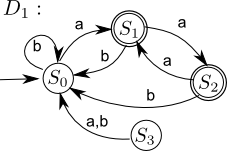
\includegraphics[width=0.3\textwidth]{img_10_1.png}
\caption{Diagrama de transición $D_1$}\label{img_10_1}
\end{figure}

$I=\{a,b\}$
%Grafico2
\begin{figure}[h!]
\centering
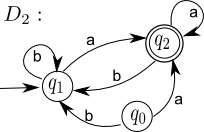
\includegraphics[width=0.3\textwidth]{img_10_2.png}
\caption{Diagrama de transición $D_2$}\label{img_10_2}
\end{figure}

\begin{center}
$\begin{array}{lp{1cm}l}
\mbox{Para }D_1:&			&\mbox{Para }D_2:	\\
S_1=\{s_0,s_1,s_2,s_3\}&		&S_2=\{q_0,q_1,q_2\}\\
s_1^*=s_0&					&s_2^*=q_1	\\
F_1=\{ s_1,s_2\}&			&F_2^=\{q_2\}
\end{array}$
\end{center}

Para $D$: 
\begin{align*}
S=&\{s_0,s_1,s_2,s_3,q_0,q_1,q_2\}\\
F=&\{s_1,s_2,q_2\}
\end{align*}

Minimizamos $D$:

Se tiene $\pi =\{P_1,P_2\}$, donde:
\begin{align*}
P_1=&\{s_1,s_2,q_2\}\mbox{	y}\\
P_2=&\{s_0,s_3,q_0,q_1\}
\end{align*}

Evaluamos $P_1$ para cada símbolo de $I$.

\begin{center}
\begin{tabular}{c|cc}
		&\multicolumn{2}{c}{$\delta$}	\\
$S\backslash I$	&$a	$			&$b$			\\ \hline
$s_1$	&$s_2\in P_1$	&$s_0\in P_2$	\\
$s_2$	&$s_1\in P_1$	&$s_0\in P_2$	\\
$q_2$	&$\downlegend{q_2\in P_1}{estados  equivalentes}$	&$q_1\in P_2$
\end{tabular}
\end{center}

Evaluamos $P_2$ para cada símbolo de $I$.

\begin{center}
\begin{tabular}{c|ccl}
		&\multicolumn{2}{c}{$\delta$}	\\
$S\backslash I$	&$a$	&$b$	&\\ \hline
$s_0$	&$s_1\in P_1$	&$s_0\in P_2$ &	\\
$s_3$	&$s_0\in P_2$	&$s_0\in P_2$ &$\rightarrow$ **	\\
$q_0$	&$q_2\in P_1$	&$q_1\in P_2$ &	\\
$q_1$	&$q_2\in P_1$	&$q_1 \in P_2$ &

\end{tabular}
\end{center}

**: No es equivalente al resto.

Refinamos la partición $\pi=\{P_1,P_2,P_3\}$
\begin{align*}
\alpha \left \{
\begin{array}{ll}
P_1=	&	\{s_1,s_2,q_2\}	\\
P_2=	&	\{s_3\}\rightarrow \mbox{este es equivalente a si mismo} \\
P_3=	&	\{s_0,q_0,q_1\}
\end{array}\right.
\end{align*}

Evaluamos $P_3$ para cada símbolo de $I$(miramos D aún), comparamos con $\alpha$.
\begin{center}
\begin{tabular}{c|cc}
				&\multicolumn{2}{c}{$\delta$}	\\
$S\backslash I$	&$a$			&$b$			\\ \hline
$s_0$			&$s_1\in P_1$	&$s_0\in P_3$	\\
$q_0$			&$q_2\in P_1$	&$q_1\in P_3$	\\
$q_1$			&$q_2\in P_1$	&$q_1\in P_3$	
\end{tabular}
\end{center}
Todos son equivalentes.

Así que ya no refinamos. Además en $P_3$, $s_0,q_1$ son equivalentes, luego $D_1$ y $D_2$ son equivalentes. El autómata equivalente a $D_1$ y $D_2$ es(Figura \ref{img_10_3}):
\begin{figure}[h!]
\centering
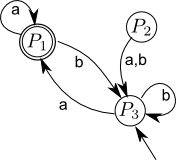
\includegraphics[width=0.3\textwidth]{img_10_3.png}
\caption{Diagrama de transición $D$}\label{img_10_3}
\end{figure}
Para el estado inicial, veo en que conjunto está incluido y ese será mi estado inicial. Veo elementos de $P_2$, y veo con que símbolo está en la primera gráfica, luego veo donde cae o (estado siguiente) y ese estado veo en que conjunto final está.

\begin{align*}
\left. \begin{array}{c}
aba \; \checkmark \\
bba \; \checkmark \end{array}\right \} \mbox{acepta} \rightarrow \mbox{pero no pasa por } P_2
\end{align*}

Se identifica que $P_2$ es un estado inaccesible, luego podemos retirarlo(Figura \ref{img_10_4}).
\begin{figure}[h!]
\centering
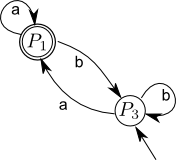
\includegraphics[width=0.3\textwidth]{img_10_4.png}
\caption{Autómata Finito Simplificado}\label{img_10_4}
\end{figure}

En un AFD: $\delta( \downlegend{s_1}{(1)},\downlegend{a}{(2)})=\downlegend{s_2}{(3)}$

donde: $\begin{array}{cl}
			(1)	& 	\mbox{Estado actual} \\
			(2)	&	\mbox{Símbolo}	\\
			(3)	&	\mbox{Estado siguiente}
\end{array}$

\section{Autómatas Finitos No Deterministas}

Si la condición que existe una única transición para el par $(s,a)$ se elimina, es decir, si para algún par $(s,a)$ hubiera transiciones hacia dos o más estados se tiene lo que se denomina, un autómata no determinístico \textbf{(AFND)}.

\begin{figure}[h!]
\centering
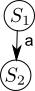
\includegraphics[width=0.05\textwidth]{img_10_5.png}
\caption{AFD}\label{img_10_5}
\end{figure}

\begin{figure}[h!]
\centering
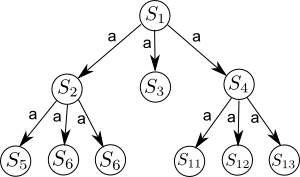
\includegraphics[width=0.5\textwidth]{img_10_6.png}
\caption{AFND}\label{img_10_6}
\end{figure}

\textbf{Definición: }Un autómata FND, $N=(S,I,\delta,s^*,F)$. $S,I,s^*$ y $F$ se definen del mismo modo que en los AFD.

\begin{center}
$\begin{array}{ll}
\delta:	&\mbox{regla de transición}	\\
\delta:	& S\times I \rightarrow P(s)	\\
P(s)	&\mbox{incluye a } \phi
\end{array}$
\end{center}

Como $\delta$ asigna a cada par de estado y símbolo, un conjunto de estados, se le denomina relación de transición.

\subsection{Representaciones para un AFND}

\begin{enumerate}
\item Tabla de transición:
	Sea el AFND $N$, donde:
	
	$\begin{array}{ll}
	S=	&\{s_0,s_1,s_2\}	\\
	I=	&\{a,b\}\rightarrow **	\\
	s^*=&s_0	\\
	F=&\{s_0\}	
	\end{array}$
	
	**: Cada estado debe tener dos salidas(normalmente). en este caso(AFND) no se cumple.
	
\textbf{Ejemplo: } Si: 

$\begin{array}{ll}
	\delta(s_0,a)=	&\{s_1\}	\\
	\delta(s_1,b)=	&\{s_0,s_2\}	\\
	\delta(s_2,a)=	&\{s_0\}
\end{array}$

Dibuje la tabla de transición:

\begin{center}
\begin{tabular}{r|cl}
	&$a$	&$b$	\\ \hline
$(1)\rightarrow \#s_0$	&$\{s_1\}$	&$\phi$	\\
$s_1$		&$\phi$	&$\{s_0,s_2\}$	\\
$s_2$		&$\{s_0\}$	&$\phi\rightarrow (2)$	
\end{tabular}
\end{center}

(1): Estado de aceptación; (2):Si no me dan información se pone $\phi$.
\item Diagrama de Transición:

\begin{figure}[h!]
\centering
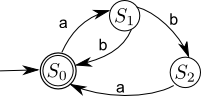
\includegraphics[width=0.3\textwidth]{img_10_7.png}
\caption{Diagrama de Transición}\label{img_10_7}
\end{figure}

\textbf{Ejercicio: }Halle el D.T del AFND siguiente:
\begin{center}
\begin{tabular}{r|cc}
	&$0$	&$1$	\\ \hline
$\rightarrow s_0$	&$\{s_0,s_1\}$	&$\{s_3\}$	\\
$s_1$				&$\{s_0\}$		&$\{s_1,s_3\}$\\
$\#s_2$				&$\{\phi\}$		&$\{s_0,s_2\}$\\
$\#s_3$				&$\{s_0,s_1,s_2\}$&$\{s_1\}$
\end{tabular}
\end{center}

\begin{figure}[h!]
\centering
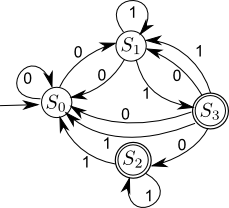
\includegraphics[width=0.3\textwidth]{img_10_8.png}
\caption{Diagrama de Transición}\label{img_10_8}
\end{figure}
\end{enumerate}

\textbf{Ejemplo: }Considere AFND: $N=(S,I,\delta,s^*,F)$. Procesemos la cadena $w=aba$, $s^*=s_0$

\begin{center}
$\begin{array}{cl}
\delta(s_0,a)=	&s_1	\\
\delta(s_1,b)=	&s_2 \rightarrow \mbox{Elijo }\{s_0,s_2\}	\\
\delta(s_2,a)=	&s_0 \rightarrow \mbox{estado de aceptación}
\end{array}$
\end{center}

Al ser $\delta(s_1,b)=s_0$ y $\delta(s_0,a)=s_1 \rightarrow w$ no es aceptada.

Pero si hay un camino que $w$ si es aceptada entonces $w$ es aceptada por AFND. $w$ es aceptada por AFND $N$.

En un modelo de computación no determinista se asume que siempre se hace la elección correcta.

\textbf{Definición: }Sea un AFND $N=(S,I,\delta,s^*,F)$. La regla de transición extendida para $N$ es una relación de $P(s)\times I^*$ hacia $P(s)$, la cual se define de forma recursiva como sigue:

\begin{itemize}
\item $\widehat{\delta}(\phi,w)=\phi$, $\forall w\in I^*$
\item $\widehat{\delta}(A,\varepsilon)=A$,  $\forall A\subseteq S$
\item $\widehat{\delta}(A,au)=\widehat{\delta}\left(\bigcup_{s\in A}\delta(s,a),u\right)$,  $A\subseteq S, a\in I, u\in I^*$

En particular cuando $w=a$ y $A\not= \phi$.
\begin{align*}
\widehat{\delta}(A,a)&=\widehat{\delta}(A,a.\varepsilon)	\\
	&=\widehat{\delta}\downlegend{\left(\bigcup_{s\in A}\delta(s,a)\varepsilon\right)}{$B=\{s_1\cup s_2\cup s_3\}$}, \\
	&=\bigcup_{s\in A}\delta(s,a)
\end{align*}
\end{itemize}

\textbf{Ejemplo: }Dado el AFND, $N$ donde:
\begin{align*}
S=&\{s_0,s_1\}	\\
I=&\{0,1\}	\\
s^*=&s_0	\\
F=&\{s_1\}
\end{align*}
\begin{center}
\begin{tabular}{c|cc}
	&$0$	&$1$	\\ \hline
$\rightarrow s_0$	&$\{s_0,s_1\}$	&$\{s_0\}$	\\
$\#s_1$	&$\phi$		&$\phi$
\end{tabular}
\end{center}
Use la función recursiva y determine si $w=1010$ es aceptada o no por $N$ en $I=\{0,1\}$.

\begin{align*}
\widehat{\delta}(\{\underbrace{s_0}_{A}\},\uplegend{1}{a}\overbrace{1010}^{u}) &=\widehat{\delta}(\delta(s_0,1),010)	\\
					  &=\widehat{\delta}(\{s_0\},\uplegend{0}{a}\overbrace{10}^{u})\\
					  &=\widehat{\delta}(\delta(s_0,0),10)	\\
					  &=\widehat{\delta}(\{s_0\},10)	\\
					  &=\widehat{\delta}(\delta(s_0,1),0)	\\
					  &=\widehat{\delta}(\{s_0\},0)	\\
					  &=\delta(\{s_0\},0)	\\
					  &=\{s_1,s_0\}
\end{align*}

Si es estado de aceptación, entonces $w$ es aceptada por $N$.

\textbf{Definición: }El lenguaje reconocido por un AFND $N$ es el conjunto:
$$L(N)=\{ w\in I^* / \widehat{\delta}(\{s^*\}, w)\cap F\not= \phi\}$$

Para afirmar que una cadena no está en $L(N)$ debemos agotar todas las posibilidades (formas posibles) de recorrer el diagrama de transición para dicha cadena.
